\chapter[Planejamento]{Planejamento}
\label{cap:planejamento}

Antes de iniciar o desenvolvimento do projeto, é necessário que sejam definidos os recursos necessários para a montagem do sistema, assim como a forma em que eles serão utilizados.
Esta seção descreve a escolha do equipamento e o projeto inicial do sistema.

\section[Escolha do equipamento]{Escolha do equipamento}

Para o desenvolvimento do projeto, foram disponibilizados, pela instituição CEFET-MG, dois manipuladores robóticos e diversos dispositivos que podem ser utilizados para seu controle.
A partir desse equipamento, e de outros disponíveis no mercado, foi decidido como o projeto seria realizado.
Os equipamentos utilizados para o projeto estão descritos a seguir:

\subsection[Manipuladores]{Manipuladores}

Os principais elementos deste trabalho são os manipuladores robóticos, portanto foi feito inicialmente um estudo sobre seu funcionamento e sobre como podem ser controlados.

Os manipuladores disponibilizados possuem diferenças físicas entre si, portanto o controle de cada um deles deve ser programado de forma independente.
Para diferenciá-los, serão denominados Manipulador Azul e Manipulador Preto.

A tabela \ref{tab:caracteristicasManipuladorAzul} apresenta as características do Manipulador Azul \cite{mentor_forward_kinematics}, enquanto a tabela \ref{caracteristicasManipuladorPreto} apresenta as características do Manipulador Preto.

\begin{table}
    \centering
    \caption{Características do manipulador robótico azul}
    \label{tab:caracteristicasManipuladorAzul}
    \begin{tabular}{|l|l|l|}
        \hline
        \textbf{Eixo} & \textbf{Movimento angular (graus)} & \textbf{Comprimento (mm)} \\ \hline
        \textbf{Eixo 0 (\textit{Waist})}            & 210 & 185 \\ \hline
        \textbf{Eixo 1 (\textit{Shoulder})}         & 180 & 165 \\ \hline
        \textbf{Eixo 2 (\textit{Elbow})}            & 230 & 150 \\ \hline
        \textbf{Eixo 3 (\textit{Left Wrist Axle})}  & 320 & 0 \\ \hline
        \textbf{Eixo 4 (\textit{Right Wrist Axle})} & 320 & 0 \\ \hline
        \textbf{\textit{Wrist Pitch}}               & 140 & - \\ \hline
        \textbf{\textit{Wrist Roll}}                & 320 & - \\ \hline
    \end{tabular}
\end{table}

\begin{figure}[H]
    \begin{minipage}{.5\textwidth}
        \centering
        \caption{Manipulador Robótico Azul}
        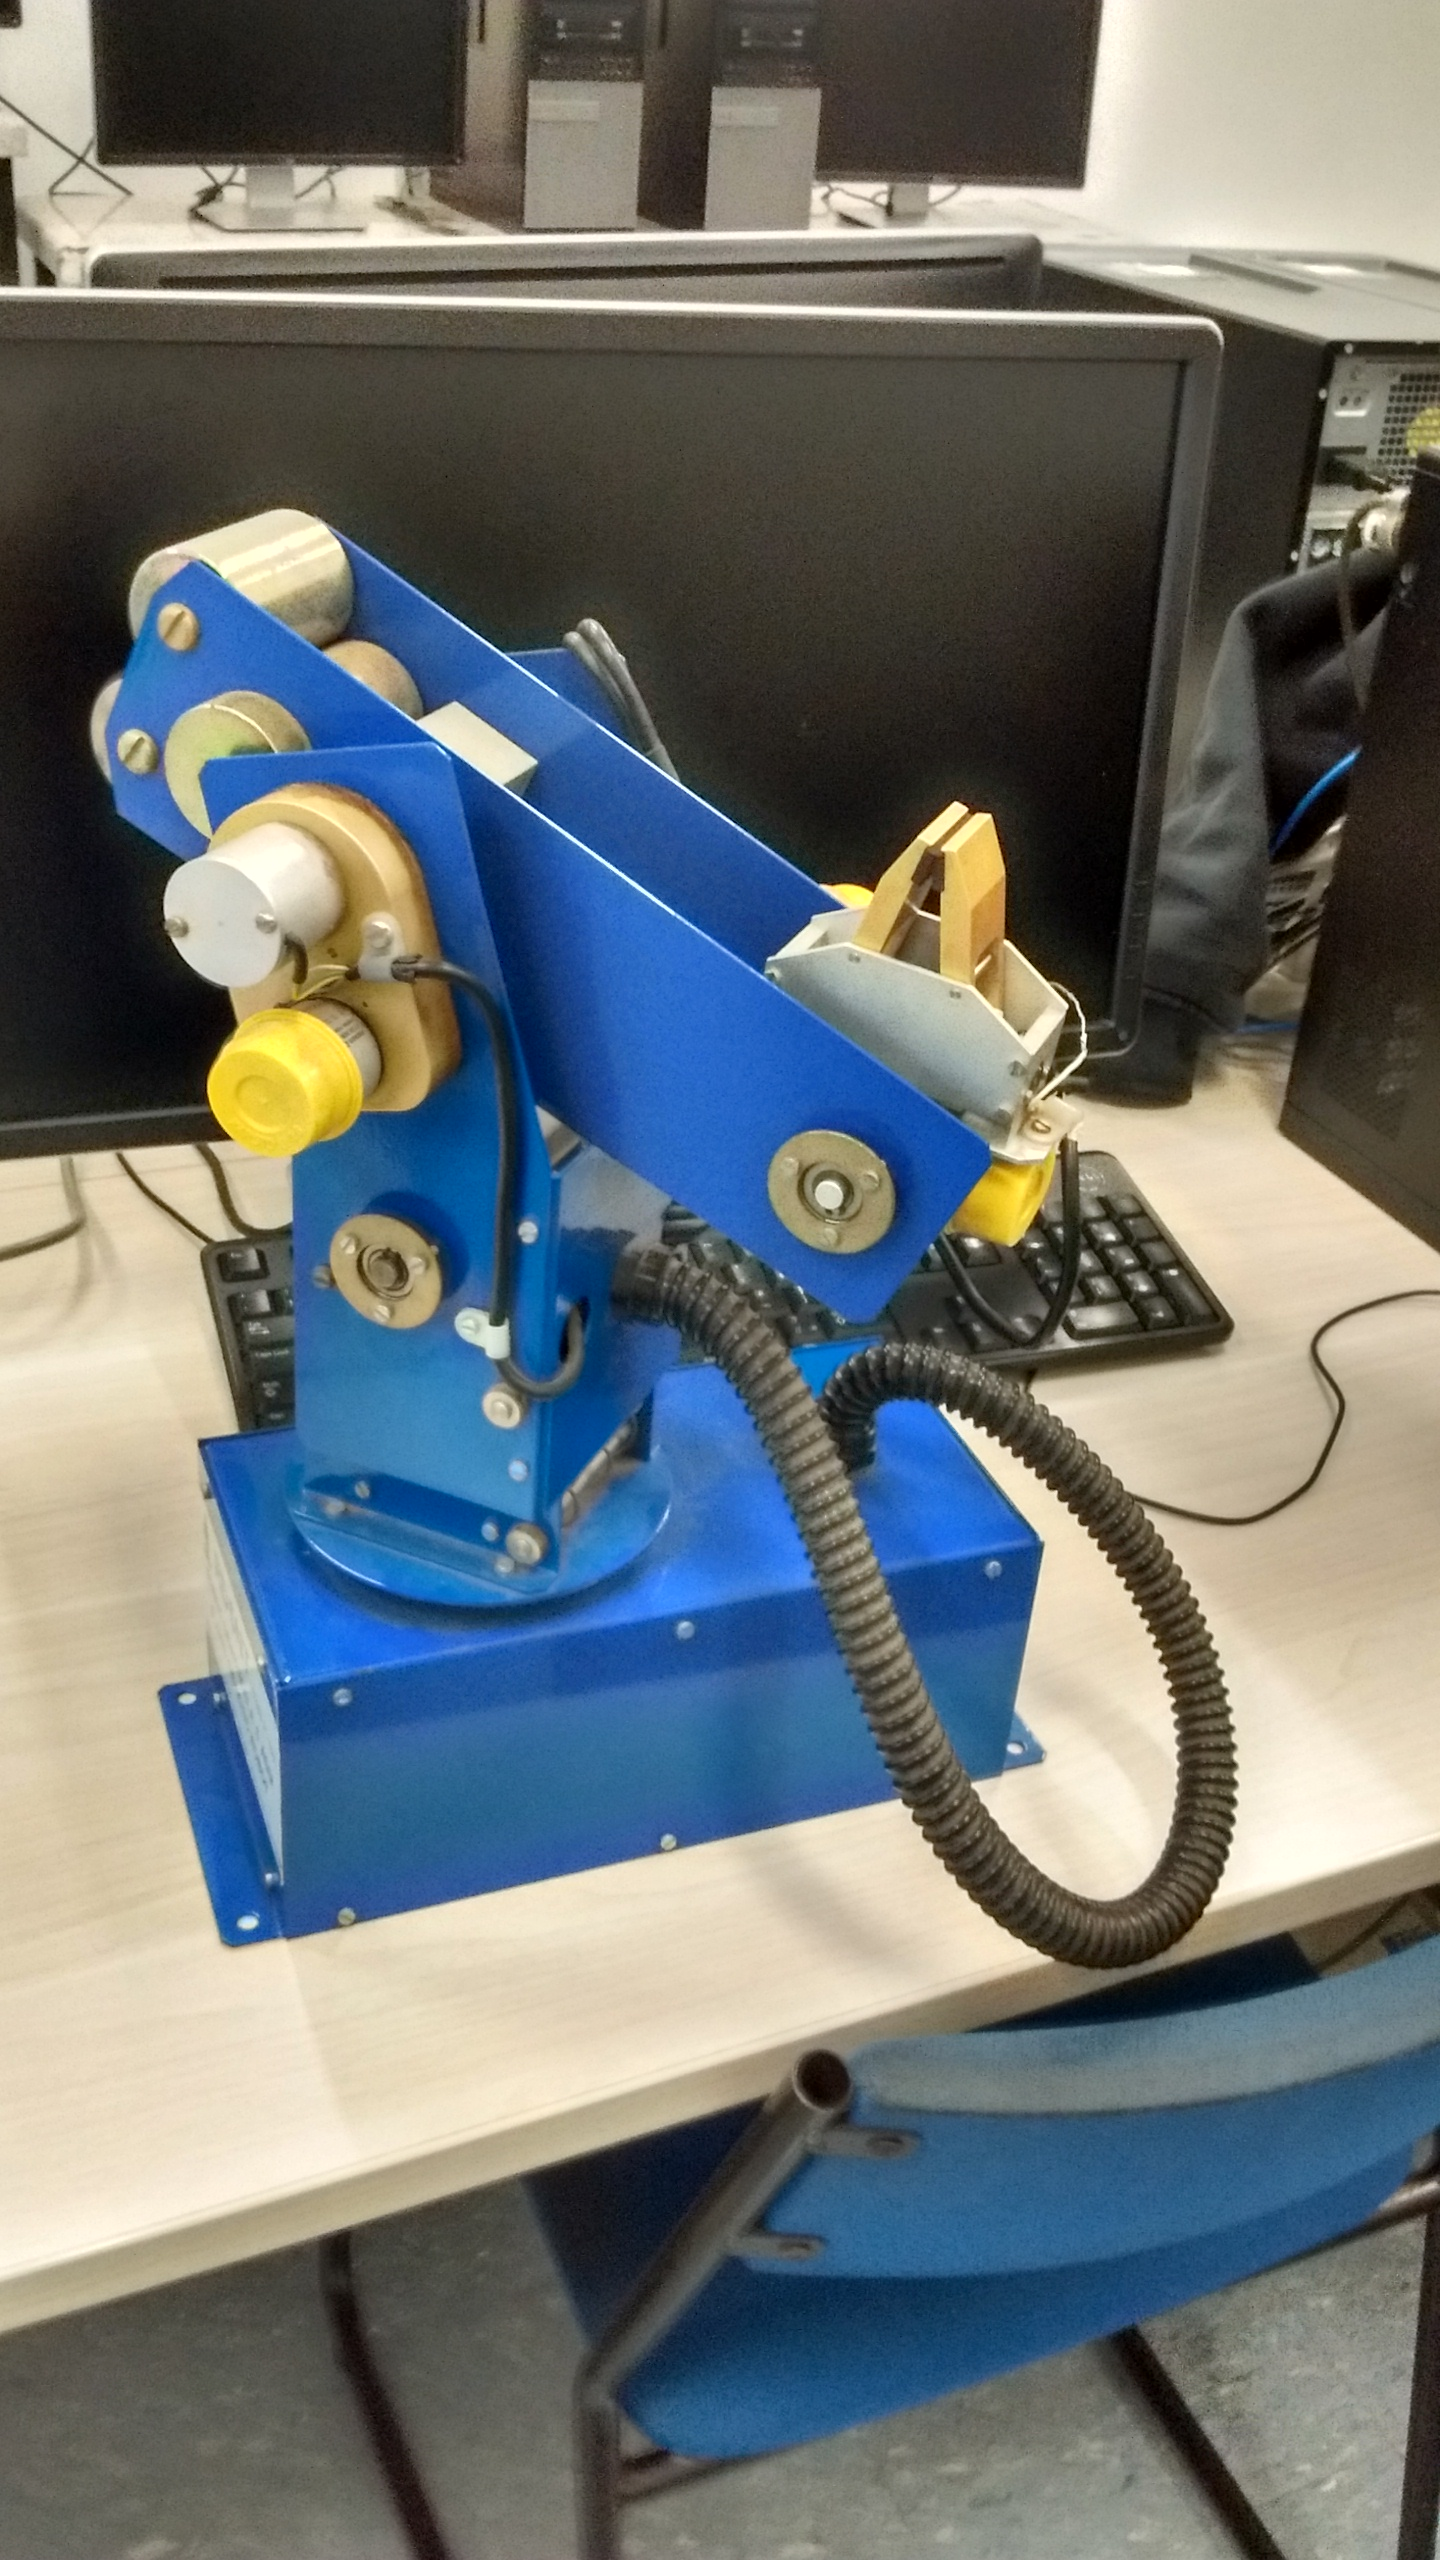
\includegraphics[keepaspectratio=true, width=0.9\linewidth]
            {img/foto-manipulador-azul.jpg}
        \fonte{http://arquivo.eng.br/robotica}
        \label{fig:fotoManipuladorAzul}
    \end{minipage}%
    \begin{minipage}{.5\textwidth}
        \centering
        \caption{Manipulador Robótico Preto}
        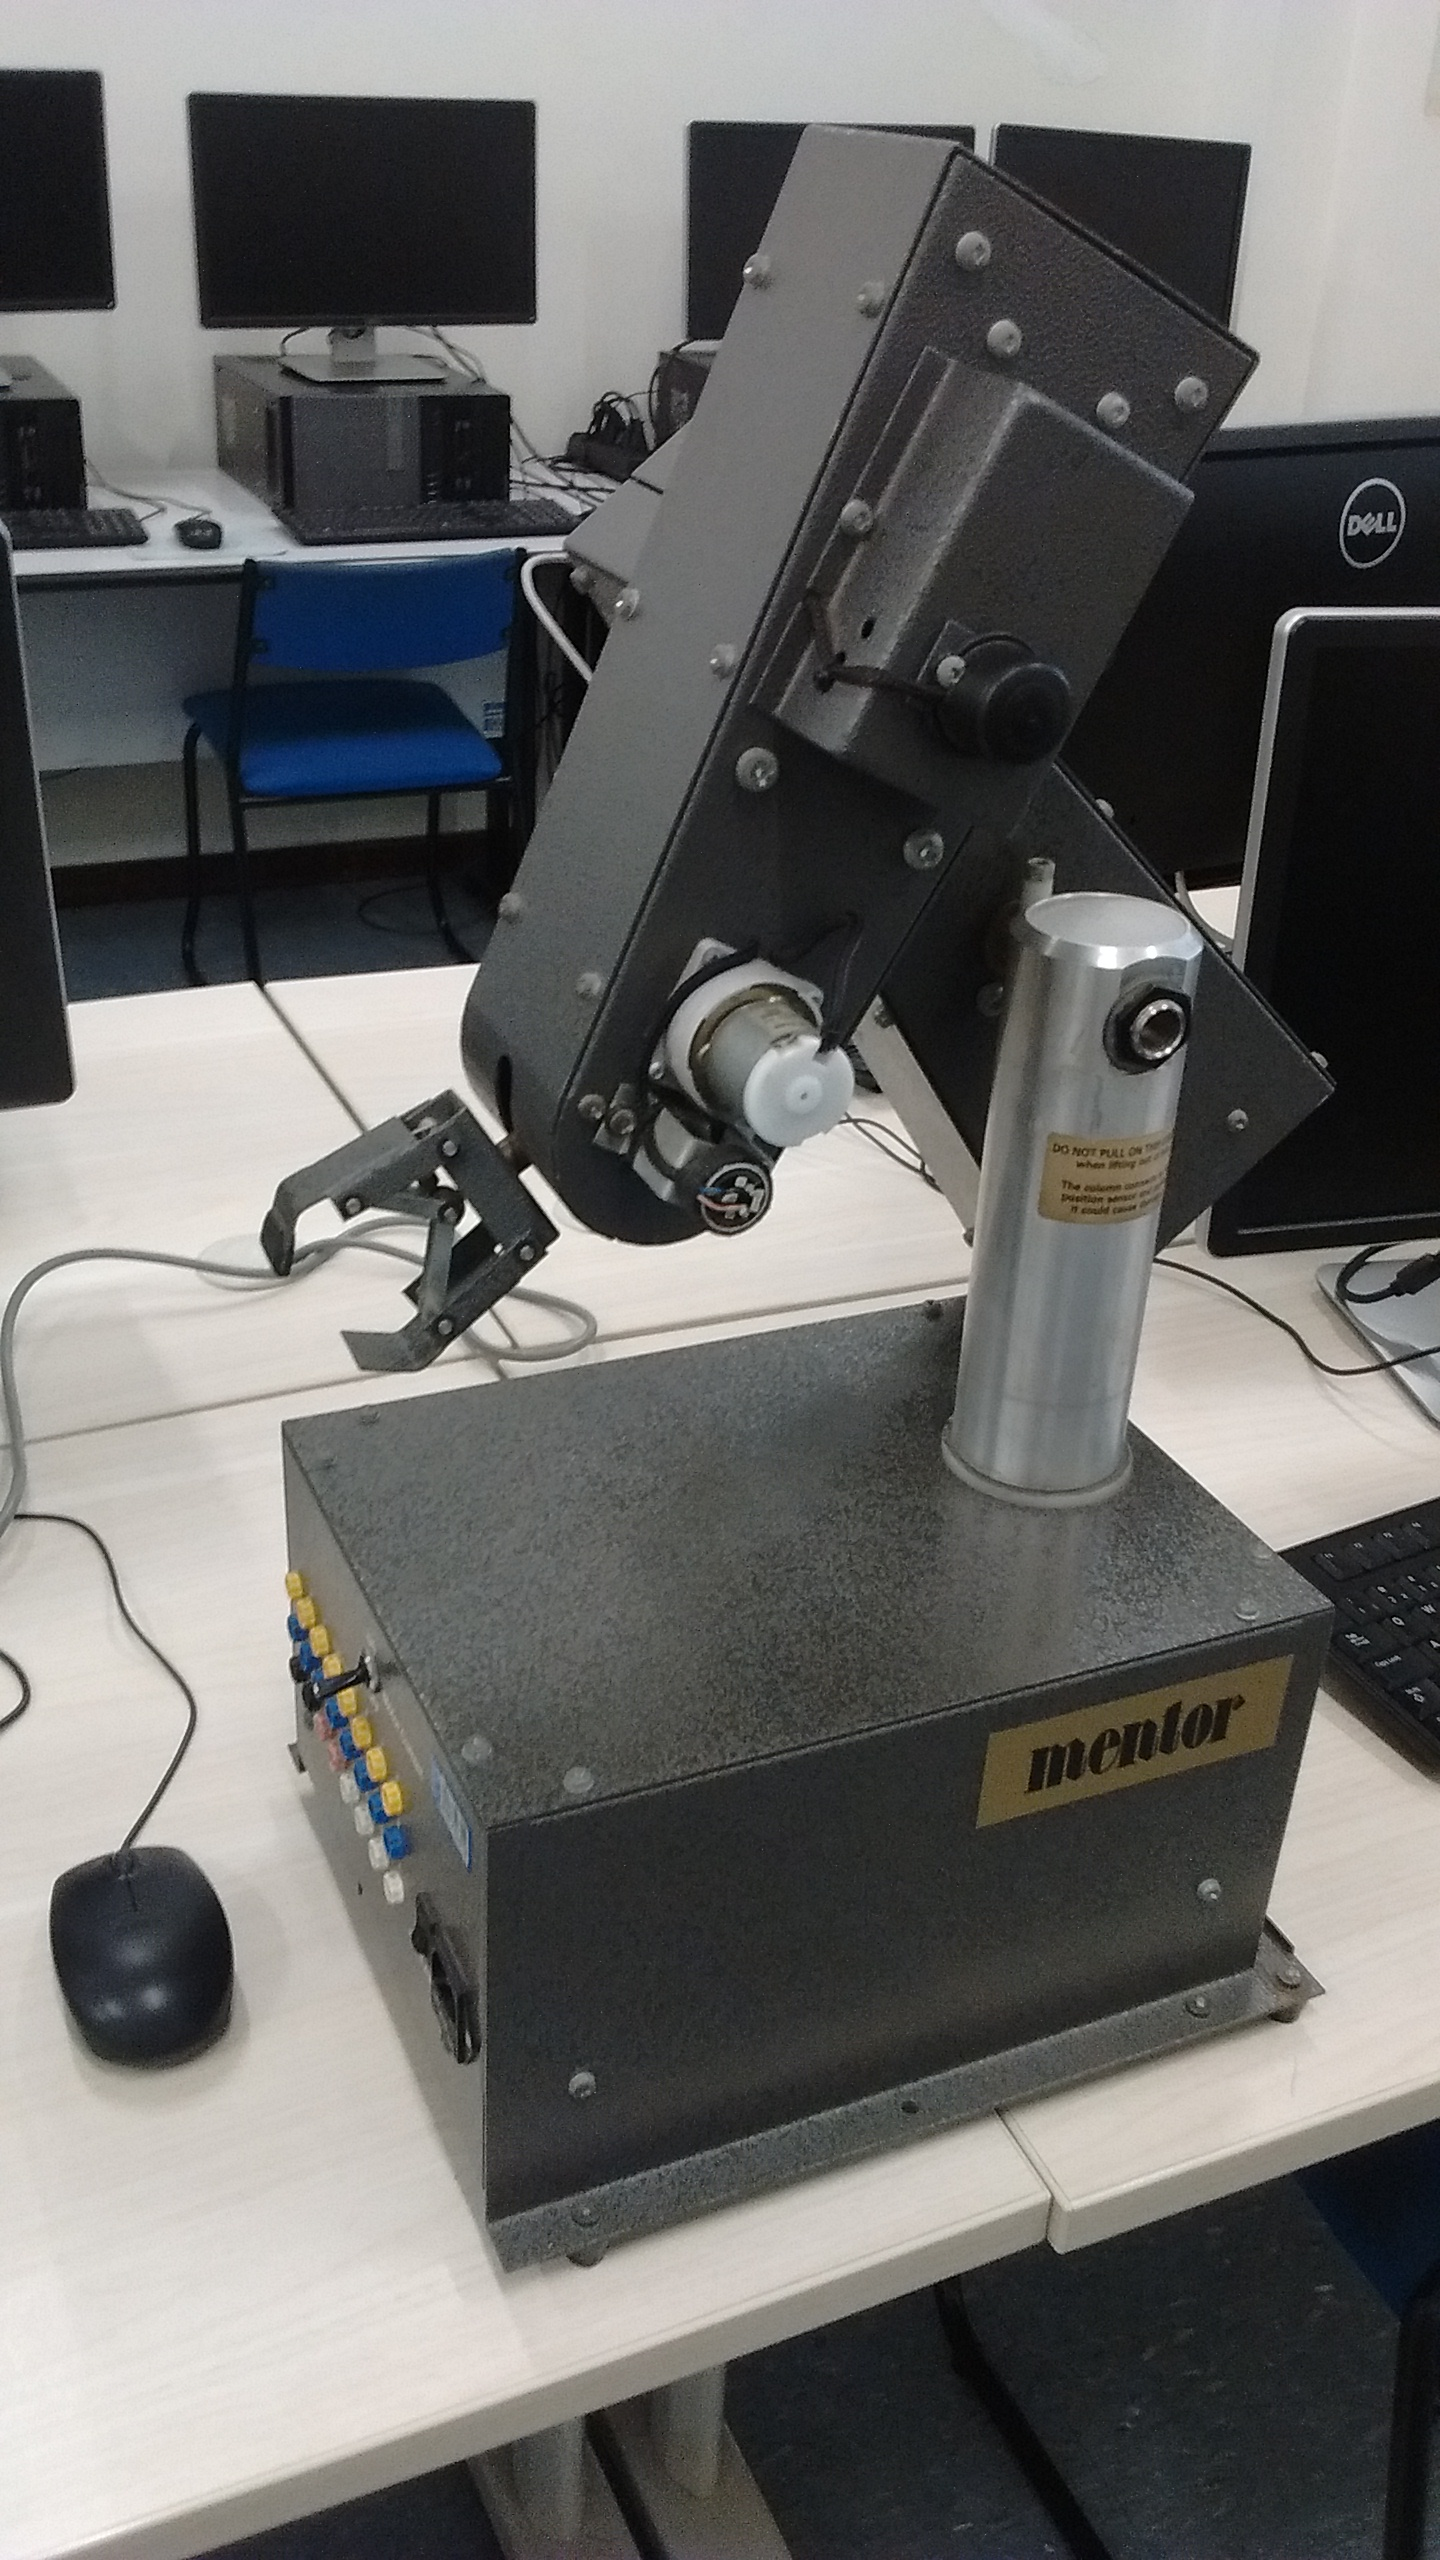
\includegraphics[keepaspectratio=true, width=0.9\linewidth]
            {img/foto-manipulador-preto.jpg}
        \fonte{http://arquivo.eng.br/robotica}
        \label{fig:fotoManipuladorPreto}
    \end{minipage}
\end{figure}

\subsection[Manete para os jogadores]{Manete para os jogadores}

Para que os jogadores possam interagir com os manipuladores, foi utilizado uma manete que possui dois \textit{joysticks} e um botão integrado a cada \textit{joystick}.
Cada jogador possui uma manete para mover seu manipulador nos eixos X e Y, e selecionar a peça que deseja mover.

\begin{figure}[H]
    \centering
    \caption{Manete para os jogadores}
    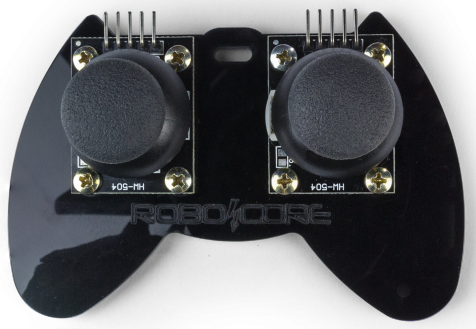
\includegraphics[keepaspectratio=true, width=0.5\textwidth]
    	{img/foto-controle-jogadores.png}
    \fonte{https://www.robocore.net/acessorios-robocore/controle-batpad}
    \label{fig:fotoManeteJogadores}
\end{figure}

\subsection[Microcontrolador]{Microcontrolador}

Para realizar a leitura dos dados das manetes e enviar os comandos para os manipuladores, foi utilizado um microcontrolador Arduino Mega 2560.
Este dispositivo deve receber sinais analógicos provenientes dos \textit{joysticks}, receber sinais digitais provenientes dos botões nos controles, receber sinais analógicos que indicam as posições dos manipuladores e enviar sinais digitais do tipo PWM para os motores dos manipuladores.

\begin{figure}[H]
    \centering
    \caption{Microcontrolador Arduino Mega 2560}
    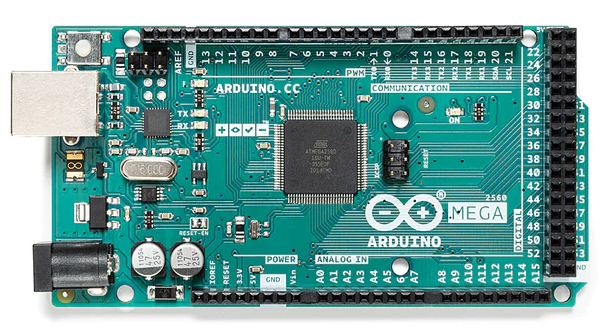
\includegraphics[keepaspectratio=true, width=0.5\textwidth]
    	{img/foto-arduino.png}
    \fonte{https://store.arduino.cc/products/arduino-mega-2560-rev3}
    \label{fig:fotoArduino}
\end{figure}

\subsection[Placa de Controle]{Placa de Controle}

Para controlar os motores dos manipuladores, é necessário o uso de uma placa de controle para converter os sinais de baixa potência provenientes do Microcontrolador em sinais de maior potência que movimentam as juntas dos manipuladores robóticos.
Essa placa deve possuir módulos de ponte H, com pelo menos 5 canais, para realizar o controle de um manipulador.

\begin{figure}[H]
    \centering
    \caption{Módulo de Ponte H}
    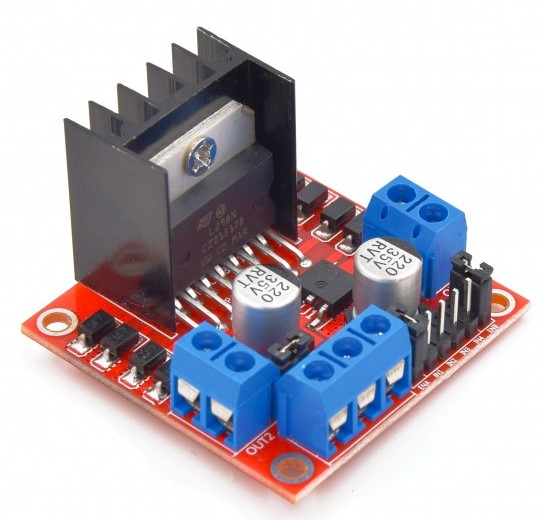
\includegraphics[keepaspectratio=true, width=0.5\textwidth]
    	{img/ponte-h.jpg}
    \fonte{https://www.smart-prototyping.com/L298N-Dual-H-bridge-Motor-Driver-Board}
    \label{fig:ponteH}
\end{figure}

\section[Projeto do sistema]{Projeto do sistema}

Com todos os equipamentos definidos, foi feito o projeto do sistema, que consiste na definição de como os dispositivos serão interligados e como o sistema irá funcionar.

O microcontrolador Arduino é a base do sistema, pois ele realiza a interligação entre os outros componentes.
A manete é conectada ao Arduino por meio de 10 cabos, sendo 5 para cada \textit{joystick} com seu respectivo botão.
A placa de controle é conectada ao Arduino por meio de 10 cabos, 2 para o controle de cada junta do manipulador robótico.
O manipulador é conectados ao Arduino por meio de 5 cabos cada para a leitura de cada ângulo dos motores.

A montagem do sistema é mostrada na Figura \ref{fig:montagemSistema}.

\begin{figure}[H]
    \centering
    \caption{Montagem do Sistema}
    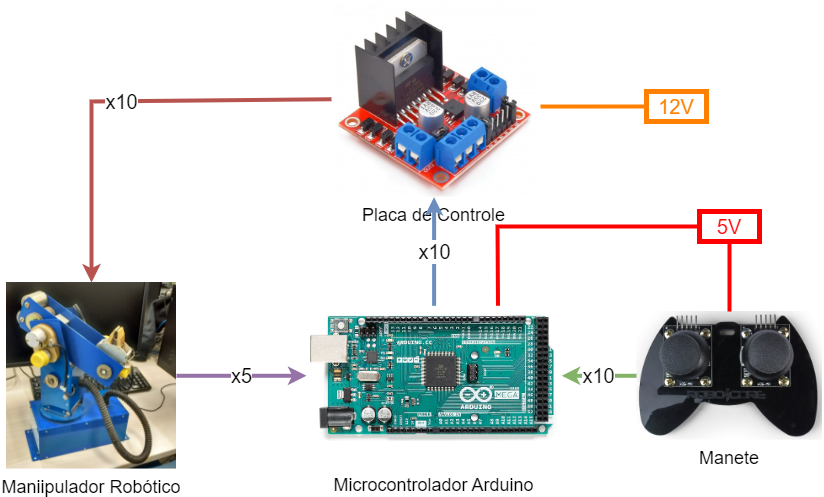
\includegraphics[keepaspectratio=true, width=0.8\textwidth]
    	{img/montagem-sistema.png}
    \fonte{Do próprio autor}
    \label{fig:montagemSistema}
\end{figure}


